% DAgger imitation-learning loop diagram

\documentclass[border=10pt,tikz]{standalone}
\usepackage{tikz}
\usepackage{xcolor}
\usetikzlibrary{arrows.meta, positioning, shapes.geometric, calc, shadows.blur}

\definecolor{slidebg}{HTML}{F8F8F8}
\pagecolor{slidebg}

\begin{document}

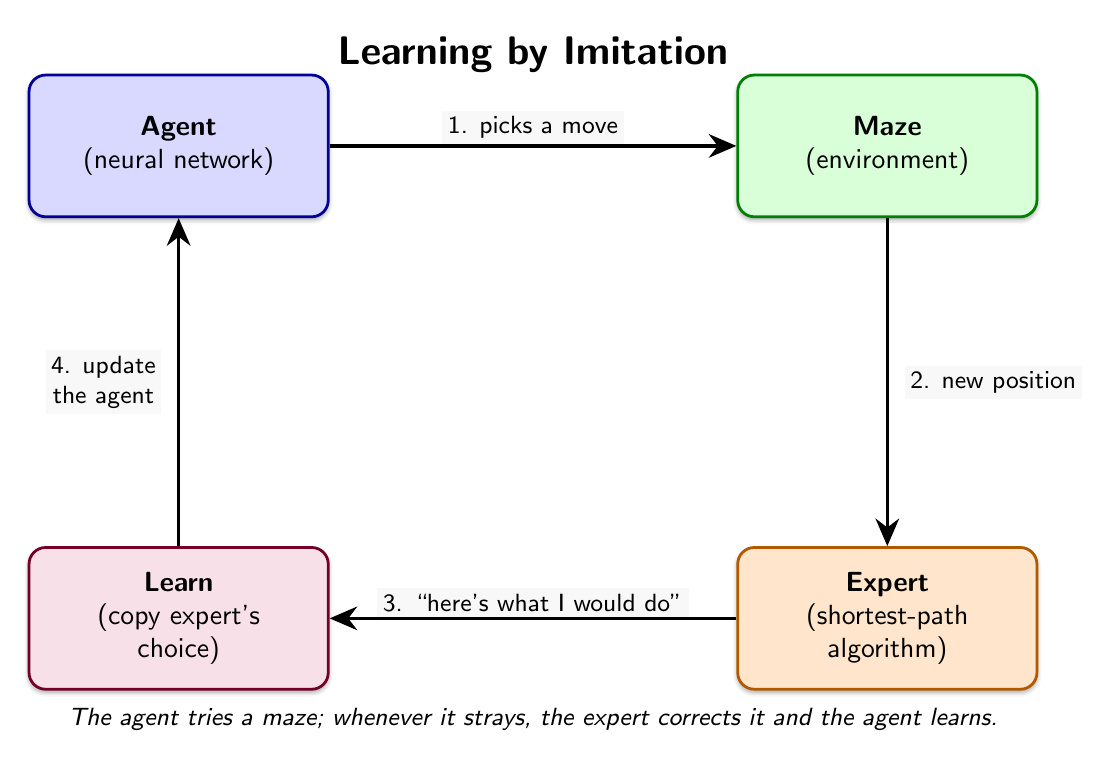
\begin{tikzpicture}[
    font=\sffamily,
    >={Stealth[length=3.5mm,width=3mm]},
    line width=1pt,
    node distance=22mm and 32mm,
    box/.style={
        rectangle, rounded corners=6pt,
        minimum width=38mm, minimum height=18mm,
        align=center, draw=black, line width=1pt,
        blur shadow={shadow blur steps=4, shadow xshift=0pt, shadow yshift=-1pt}
    },
    agent/.style={box, fill=blue!15, draw=blue!60!black},
    expert/.style={box, fill=orange!20, draw=orange!70!black},
    env/.style={box, fill=green!15, draw=green!50!black},
    learn/.style={box, fill=purple!12, draw=purple!60!black},
    arr/.style={->, line width=1.2pt},
    lbl/.style={font=\sffamily\small, align=center, fill=slidebg, inner sep=2pt}
]

% Nodes arranged in a loop
\node[agent]  (A) at (0,0)        {\textbf{Agent}\\(neural network)};
\node[env]    (E) at (9,0)        {\textbf{Maze}\\(environment)};
\node[expert] (X) at (9,-6)       {\textbf{Expert}\\(shortest-path\\algorithm)};
\node[learn]  (L) at (0,-6)       {\textbf{Learn}\\(copy expert's\\choice)};

% Loop arrows
\draw[arr] (A.east) -- node[lbl, above] {1. picks a move} (E.west);
\draw[arr] (E.south) -- node[lbl, right=2mm] {2. new position} (X.north);
\draw[arr] (X.west) -- node[lbl, above] {3. ``here's what I would do''} (L.east);
\draw[arr] (L.north) -- node[lbl, left=2mm] {4. update\\the agent} (A.south);

% Title
\node[font=\sffamily\Large\bfseries, above=8mm of $(A)!0.5!(E)$]
    {Learning by Imitation};
\node[font=\sffamily\small\itshape, below=10mm of $(X)!0.5!(L)$]
    {The agent tries a maze; whenever it strays, the expert corrects it and the agent learns.};

\end{tikzpicture}

\end{document}
